\section{Points of Interest Module}

\subsection{UML Class Diagram}

\begin{figure}[!htb]
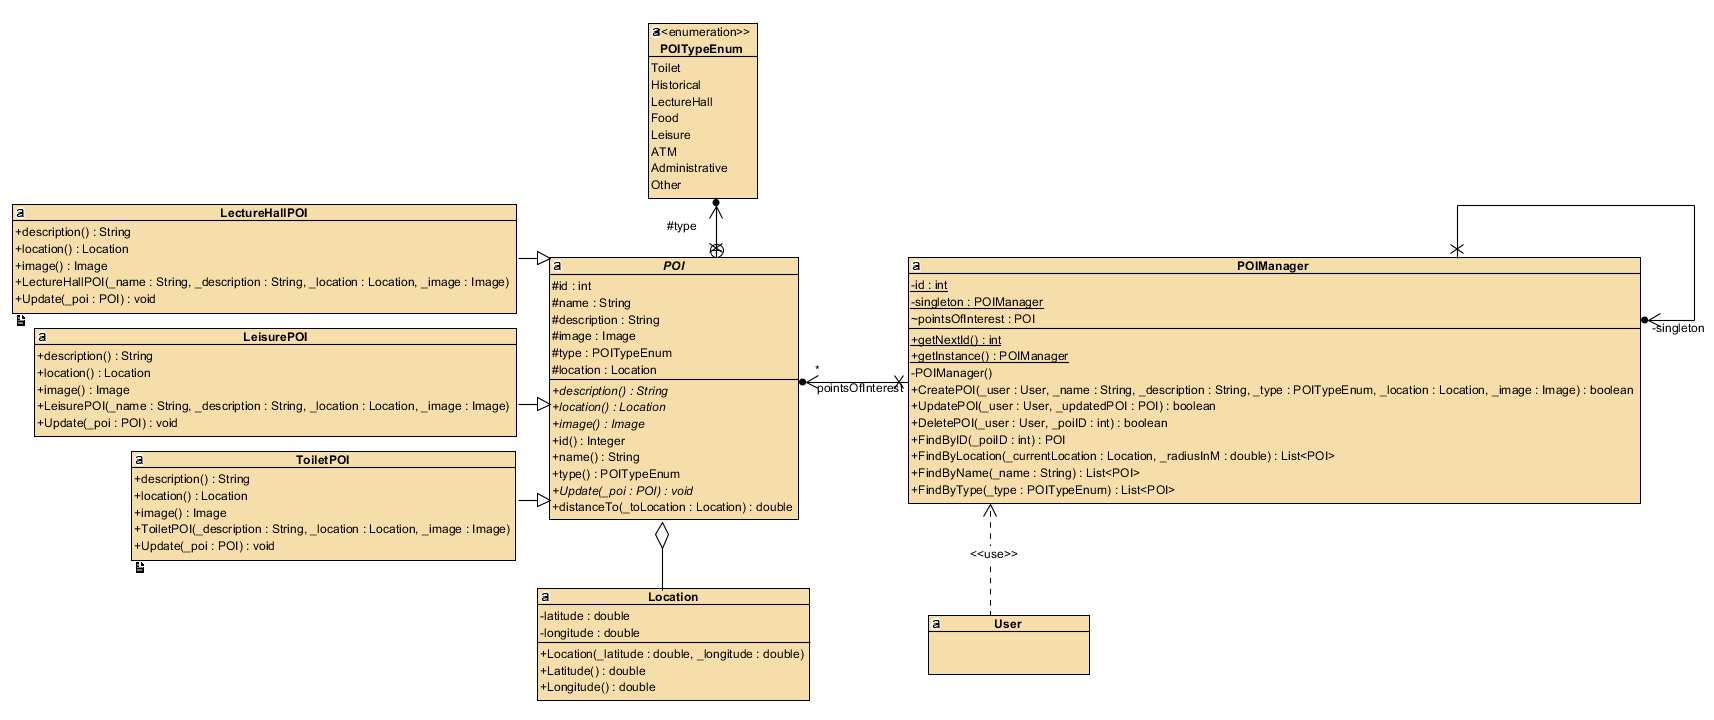
\includegraphics[width=\textwidth]{Images/ClassDiagram.png}
\caption{Class Diagram for the Points of interest module}
\end{figure}

\subsection{Use Case Diagram}

\begin{figure}[!htb]
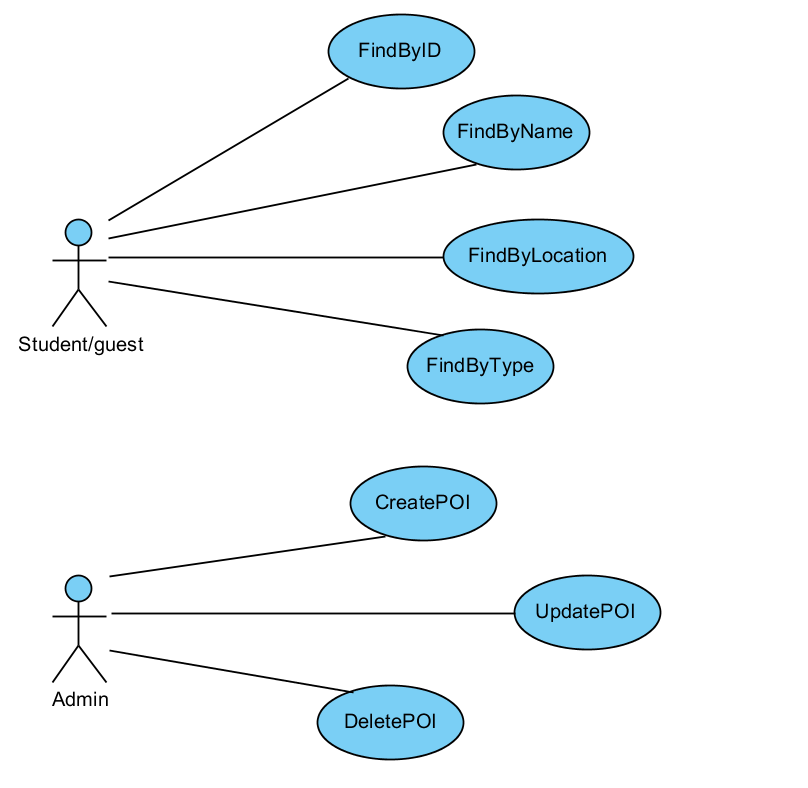
\includegraphics[width=\textwidth]{Images/UseCase.png}
\caption{Use Case Diagram for the Points of interest module}
\end{figure}

\subsection{Architectural Design of Module}

\paragraph{}The Points of Interest module will be used to persist and deliver data regarding locations that a user 
might find of interest. It will interact with the Events module, as well as the GIS module in order to retrieve and 
save it geographical location.

\paragraph{}One can assume that different types of Points of Interest(POI) will have different fields, constraints 
and requirements, therefore the POI module will make use of the factory design pattern, in order to create objects 
without exposing the creation logic to the client and allow us to refer to the newly created object using a common interface.

\paragraph{}The Points of Interest Manager class will make use of the Singleton design pattern to ensure that only one 
instance of the class exists, it will also act as the factory class to the points of interest class.

\paragraph{}At the core a Point of Interest object will have a location, description, unique id, type, name and image. 
The concrete object will then be able to impose additional attributes and constraints, such as Gender for bathrooms for 
example.

\paragraph{}Finally, the abstract point of interest class will be equipped with a stringify function to get a JSON 
representation of the object. 

\subsection{Technologies Used}

\paragraph{}It can be assumed that different types of Points of Interest will have different fields, constraints and 
requirements, therefore a traditional relational database will not be suitable for this type of data. Hence we will 
rather go for a document-oriented database like MongoDB, as the database server.

\paragraph{}The Points of Interest CRUD functions will be exposed as Simple Object Access Protocol (SOAP) web services, 
using ASP.NET core and Entity framework carrying a JSON payload.

\paragraph{}The logic of the module will be written in .NET.


\subsection{Non-Trivial Implementation Tasks}

\paragraph{}The point of interest module will be called in two ways. Firstly, by administrative user who would be able to add, remove and 
update points of interest around campus. Secondly, students and guests will be able to use it, by searching for specific locations by name,
type of location, specific areas etc. Lastly the points of interest classes SearchByLocation function will be called by the navigation module,
as the user navigates campus.

\begin{figure}[!htb]
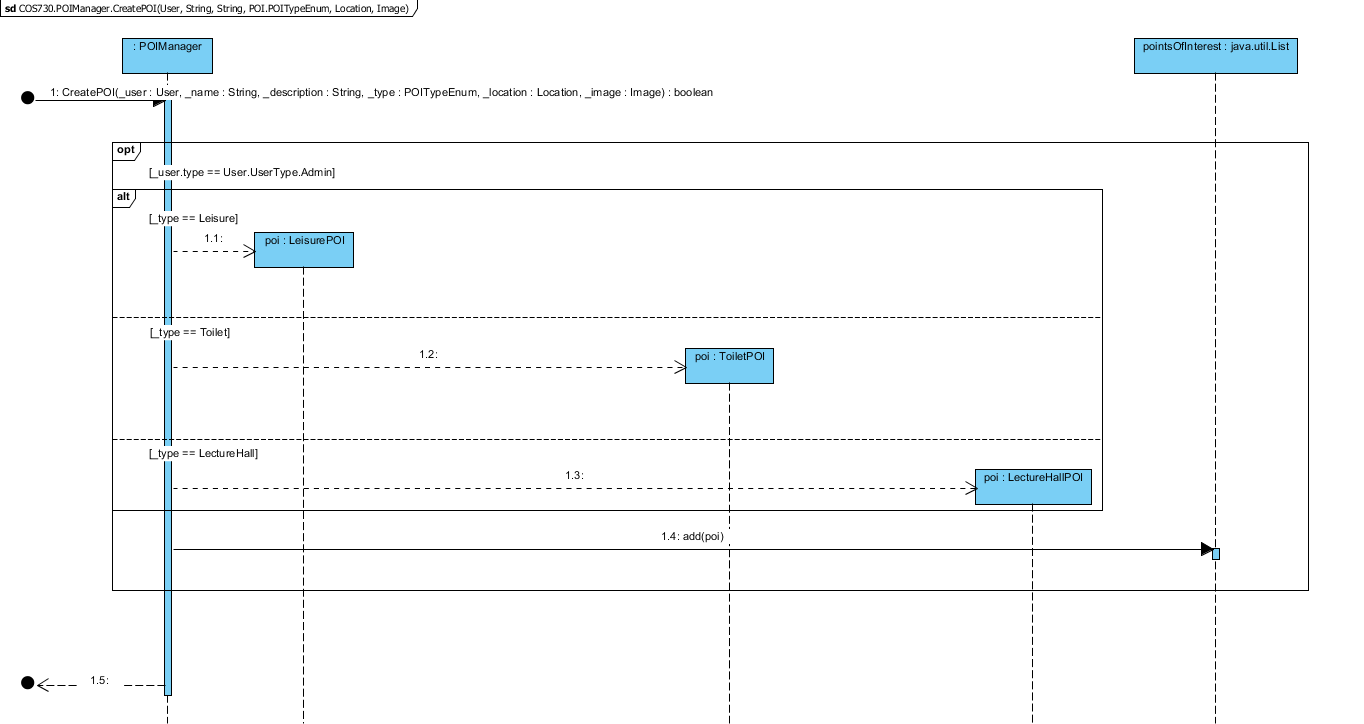
\includegraphics[width=\textwidth]{Images/CreatePOI_Sequence.png}
\caption{Sequence Diagram for the CreatePOI function}
\end{figure}

\begin{figure}[!htb]
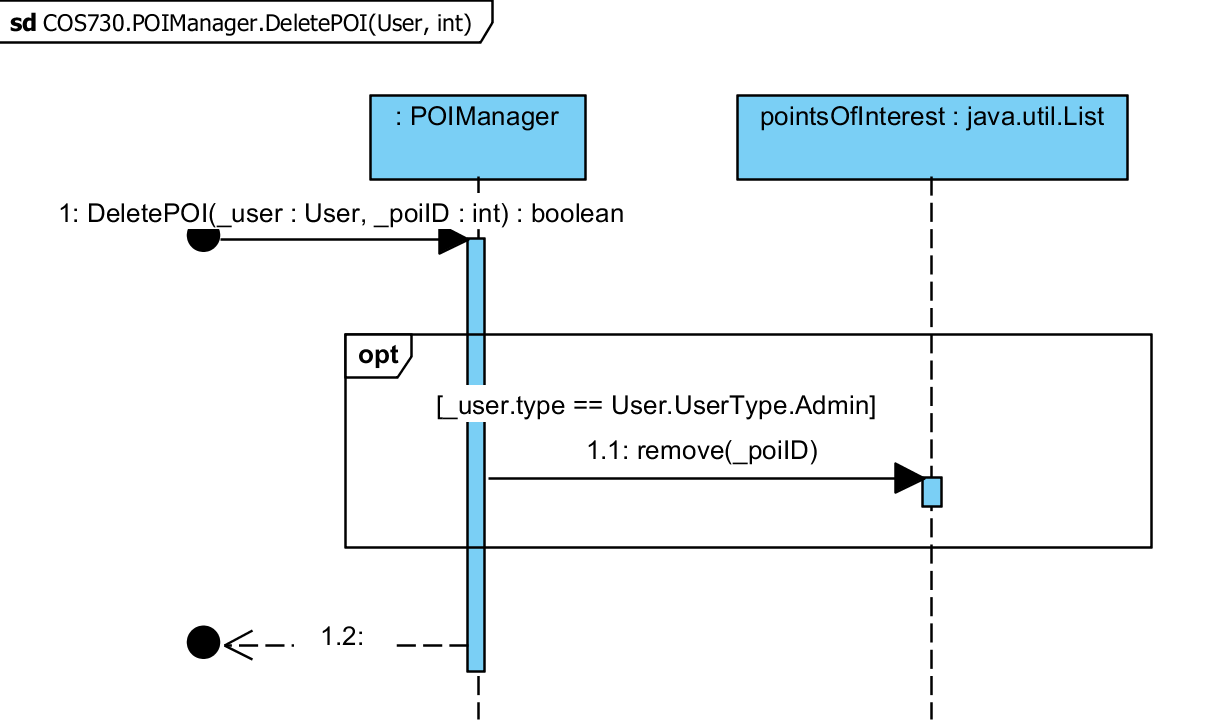
\includegraphics[width=\textwidth]{Images/DeletePOI_Sequence.png}
\caption{Sequence Diagram for the DeletePOI function}
\end{figure}

\begin{figure}[!htb]
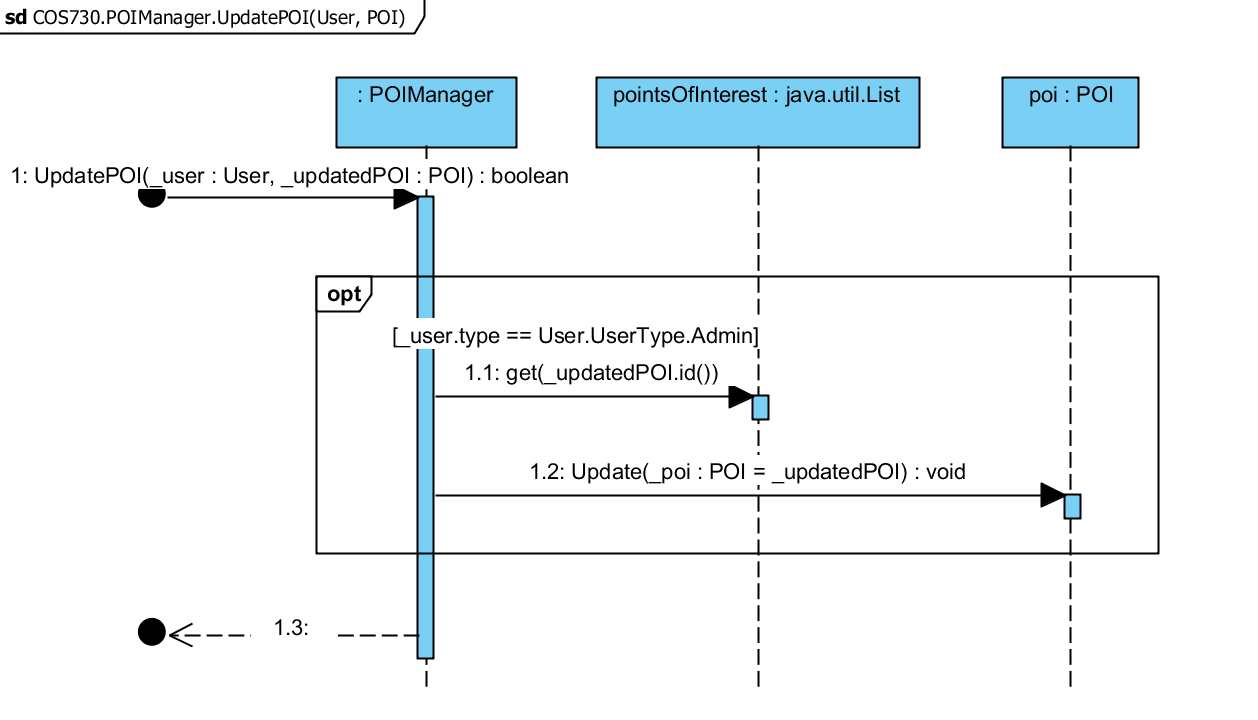
\includegraphics[width=\textwidth]{Images/UpdatePOI_Sequence.png}
\caption{Sequence Diagram for the UpdatePOI function}
\end{figure}

\begin{figure}[!htb]
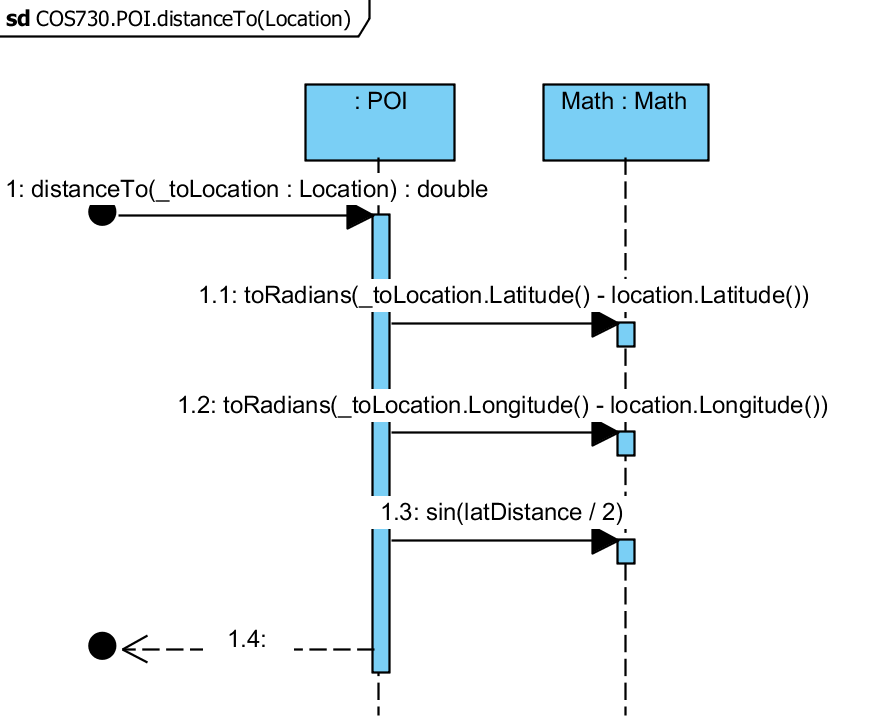
\includegraphics[width=\textwidth]{Images/DistanceTo_Sequence.png}
\caption{Sequence Diagram for the DistanceTo function}
\end{figure}

\begin{figure}[!htb]
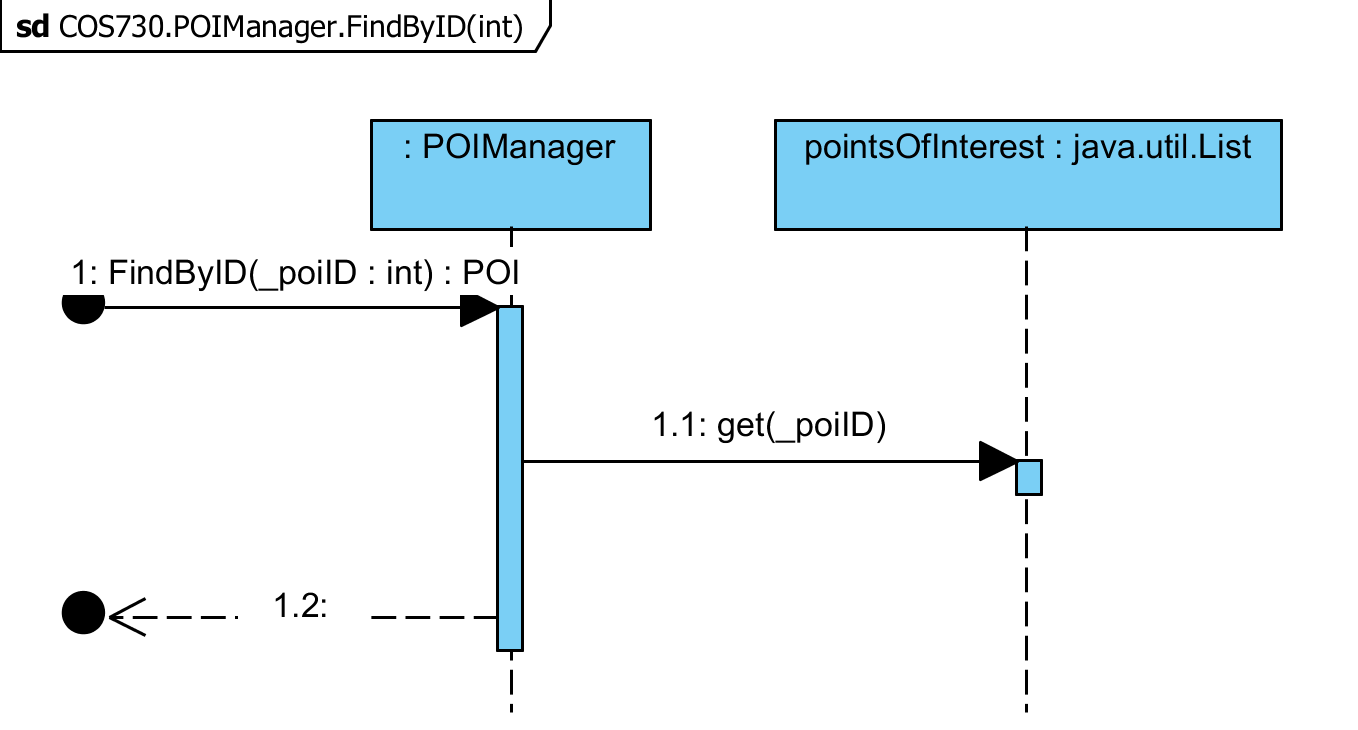
\includegraphics[width=\textwidth]{Images/FindByID_Sequence.png}
\caption{Sequence Diagram for the FindByID function}
\end{figure}

\begin{figure}[!htb]
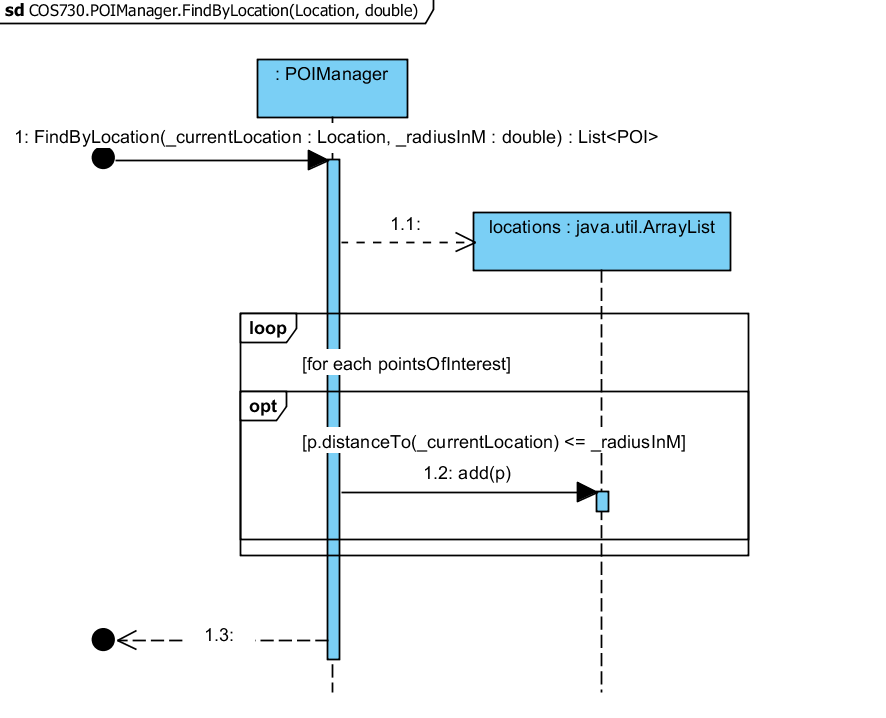
\includegraphics[width=\textwidth]{Images/FindByLocation_Sequence.png}
\caption{Sequence Diagram for the FindByLocation function}
\end{figure}

\begin{figure}[!htb]
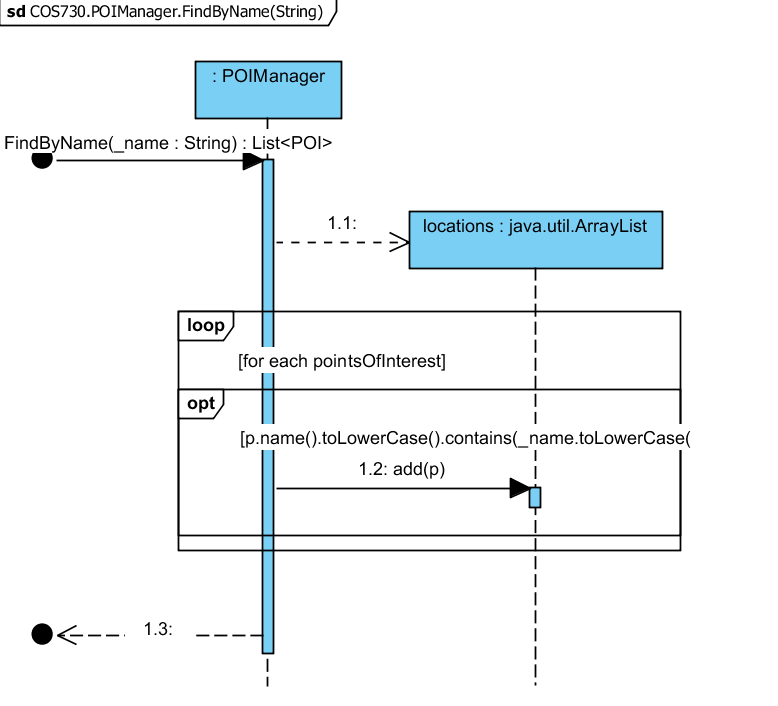
\includegraphics[width=\textwidth]{Images/FindByName_Sequence.png}
\caption{Sequence Diagram for the FindByName function}
\end{figure}

\begin{figure}[!htb]
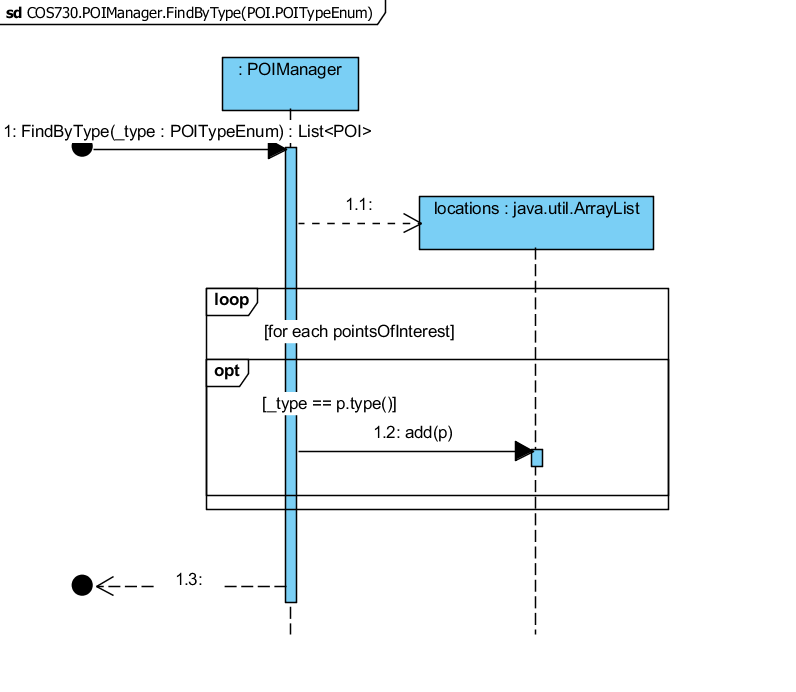
\includegraphics[width=\textwidth]{Images/FindByType_Sequence.png}
\caption{Sequence Diagram for the FindByType function}
\end{figure}

\begin{figure}[!htb]
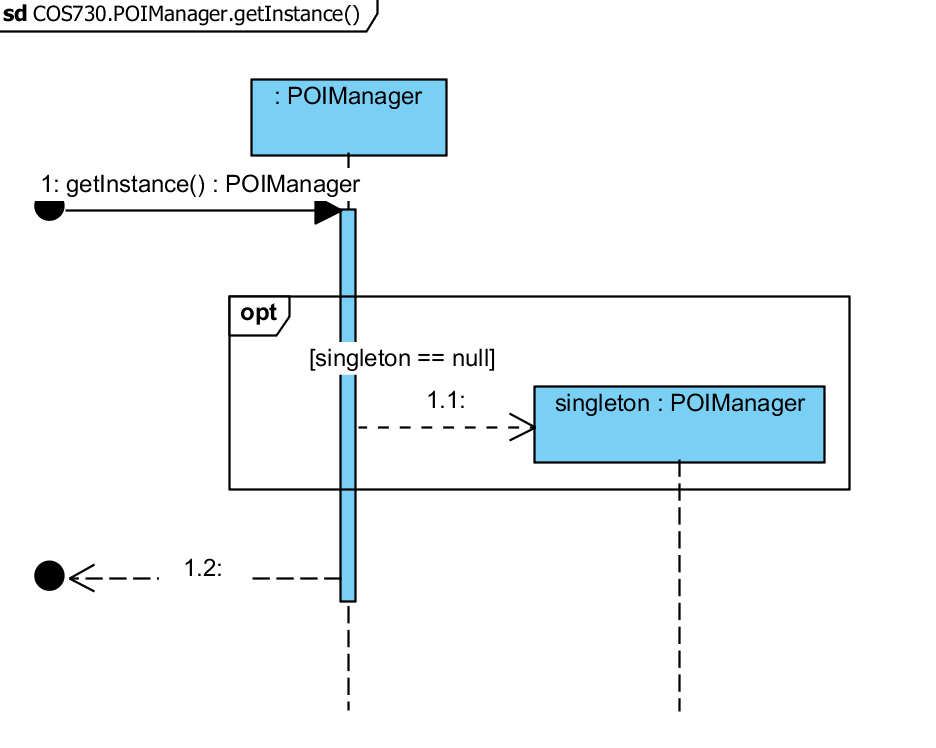
\includegraphics[width=\textwidth]{Images/getInstance_Sequence.png}
\caption{Sequence Diagram for the getInstance function}
\end{figure}
